%=====================================================
%====== If you are new to LaTeX, this website ========
%======     will be your new best friend:     ========
%======   http://en.wikibooks.org/wiki/LaTeX  ========
%======   Template created by Jonathan Blair  ========
%=====================================================



%=====================================================
%============ Controls ===============================
%=====================================================

%\documentclass[12pt,letterpaper,onecolumn]{article}
\documentclass[11pt,letterpaper,onecolumn]{article}
%\documentclass[10pt,letterpaper,onecolumn]{article}  % not recommended
%\documentclass[12pt,letterpaper,twocolumn]{article}
%\documentclass[11pt,letterpaper,twocolumn]{article}
%\documentclass[10pt,letterpaper,twocolumn]{article}


\usepackage{amsmath}
\usepackage{graphicx}
\usepackage{url}
\usepackage{textgreek}
\usepackage{float}
\usepackage{booktabs}
%\graphicspath{{path-to-folder-containing-necessary-graphics}{other folder as necessary}}


%=====================================================
%============ \begin{document} =======================
%=====================================================

\begin{document}

%=====================================================
%============ Title ==================================
%=====================================================

\title{\bf Observation of the Properties and Behavior of a Basic Transistor Switch}
%\title{\Large\bf Larger, Bolded Title}

%=====================================================
%============ Author =================================
%=====================================================
\author{
 Jairo Portillo \\*
  \\*
 PHY 338K Electronic Techniques \\*
 Department of Physics \\*
 The University of Texas at Austin \\*
 Austin, TX 78712, USA
}
\date{February 18, 2016}

%\address{The University of Texas, Austin, Texas, 78712}

\maketitle

%=====================================================
%============ Abstract ===============================
%=====================================================

\begin{abstract}

In this lab, we will explore the properties of junction transistors and how they influence the flow of signal within a circuit. We will check the current gain of the transistor and we will observe the switching action it performs as the voltage is changed. We will then observe this behavior on the oscilloscope in order to find the voltage gain and the voltage offset where switching occurs.       

\end{abstract}

%=====================================================
%============ Body of the article ==========================
%=====================================================

%=====================================================
%============ Section ==================================
%=====================================================

\section{Preperation}

In order to prepare for this lab, we must review the behavior of transistors. A transistor possess a collector, an emitter, and a base connection. In a npn transistor, the collector is more positive than the emitter while in a pnp transistor the emitter is more positive than the collector. The base-emitter and base-collector circuits behave like diodes where the base-emitter behaves as a forward bias diode and base-collector behaves as a reverse bias diode. With this behavior, it can bee seen that the collector current $I_C$ is proportional to the base current $I_B$ by a factor of the current gain $\beta$.

$$\beta=\frac{I_C}{I_B}$$

\section{Lab work}

\subsection{Apparatus}

This lab will use a signal generator, an oscilloscope, a DC voltage source, a npn transistor, a 1k$\Omega$ and 10k$\Omega$ resistors. The AC signal generator will be in series with the 10k$\Omega$ resistor and the base of the transistor. A Tee connector will connect the input AC signal with channel 1 on the oscilloscope. The emitter will be grounded and the collector will be connected to he 1k$\Omega$, channel 2, and the DC voltage source. The DC voltage source will also behave as our ground. 

\subsection{Data Collection}

In order to check the current gain $\beta$, we used the digital multimeter. For out npn transistor we found $\beta$ to be 182. We then setup the circuit as described in the Apparatus. As the voltage increased from the signal generator, the collector voltage began to decrease.This means as transistor turned on, it redirects the signal to the emitter into ground.  

\begin{figure}[H]
    \centering
    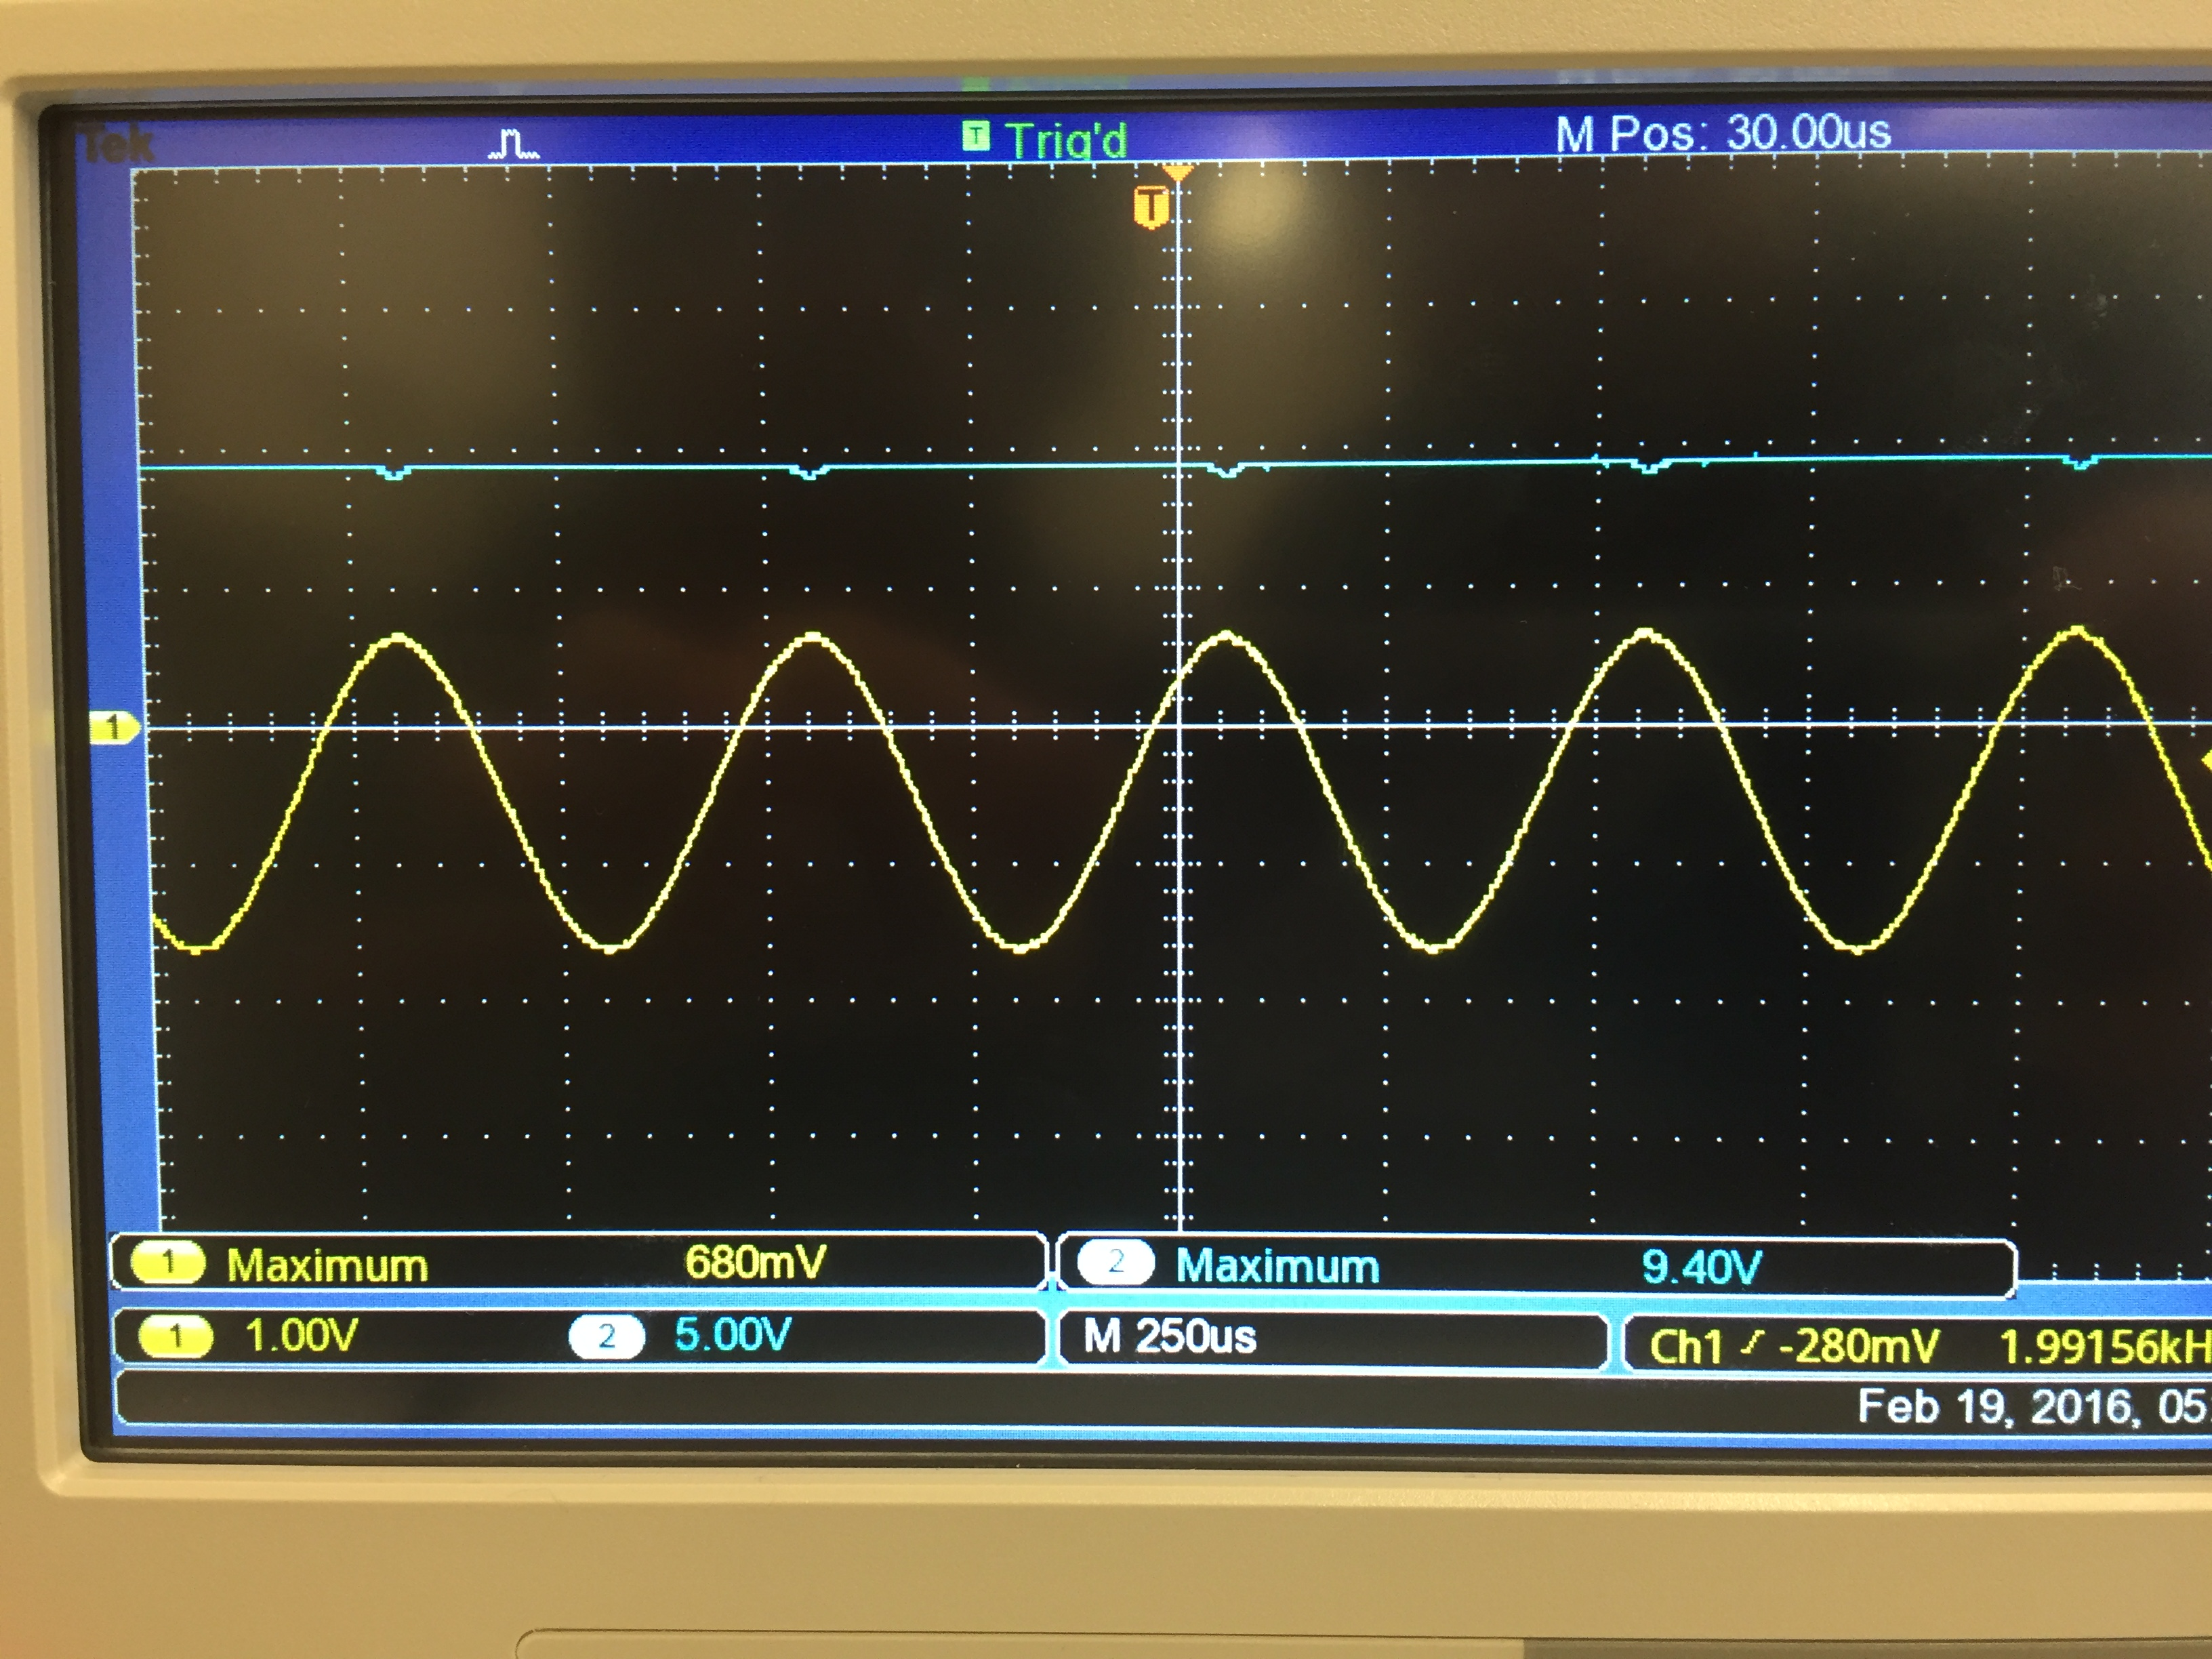
\includegraphics[scale = 0.1]{IMG_1046.JPG}
    \caption{Image of Oscilloscope of the base voltage where switching occurs.}
    \label{fig:prtd}
\end{figure}

In Figure 1, we can see that as we slightly vary the DC offset of the signal generator in order to find the base voltage of where the transistor begins to switch. The base voltage where switching occurs is 680mV which is 20mV of the expected 0.7V. In order to measure the voltage gain of the amplifier we had to use the -20dB attenuation of the signal generator to get a clear sine wave. This was due to the signal being driven too high causing the signal to be a square wave. This effect has greater effects due to the slight capacitance in the transistor. We found that the voltage gain to be 7.536 for our circuit. We then compared the measured base current to the calculated base current. Using the digital multimeter, we found the base current to me 57.3$\mu$A and using the equation   
$$I_b = \frac{V_b-V_{be}}{R_b}$$

where $I_b$ is the base current, $V_b$ is the base voltage which we measured to be 1.335V, $V_{be}$ is the voltage across the base and emitter which we measured to be 0.713V, and $R_b$ is the base resistance which was $9.8\Omega$.This gives us a base current of $63.54\mu A$. These values are $10\%$ from each other. We were unable to measure the characteristc plot as we could not figure a way to keep the base current or the base-emitter voltage constant relative to the collector current. 

\section{Summary and conclusions}

In this lab, we have seen how transistors can switch and block signals. We can see from Figure 1 that at a base voltage of 680mV the transistor begins to switch and our transistor has a current gain $\beta$ of 182. We also observed that without attenuation the transistor outputs a square wave while with attenuation it outputs a sine wave. We found that the measured and calculated base currents were $10\%$ of each other. 



%=====================================================
%============ Bibliography  ==============================
%=====================================================



%=====================================================
%============ End ====================================
%=====================================================

\end{document}

%=====================================================
%============ End ====================================
%=====================================================